\documentclass[tikz,border=5pt]{standalone}
\usepackage{lmodern}
\begin{document}
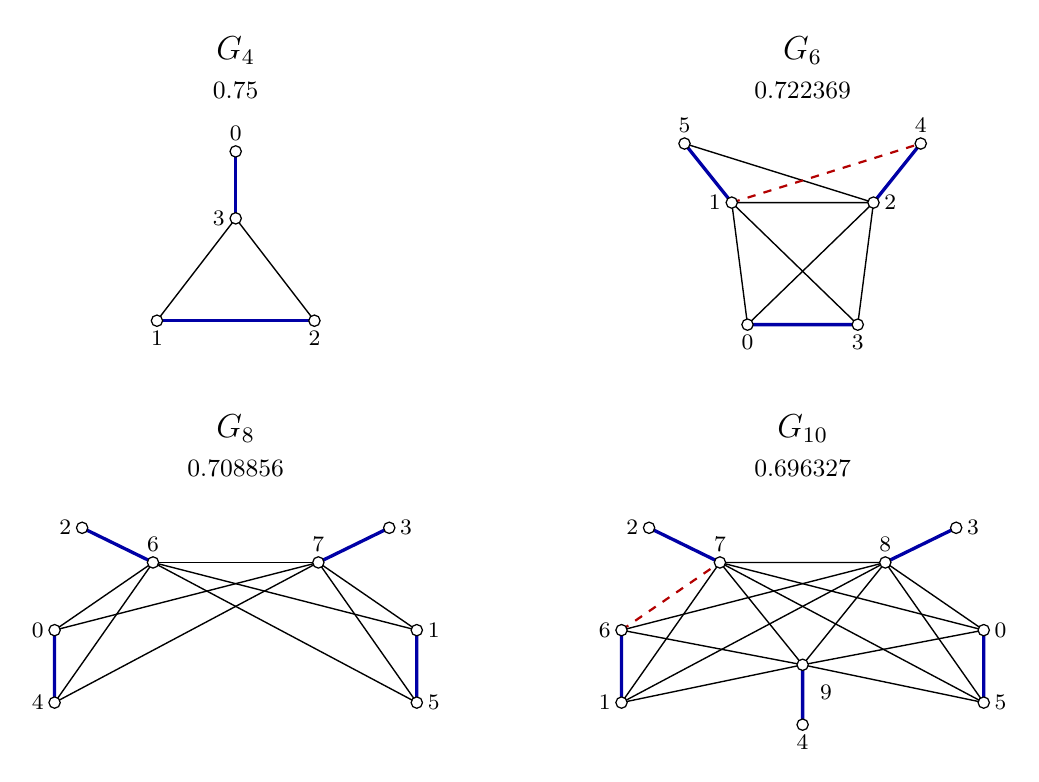
\begin{tikzpicture}[
  vertex/.style={circle,draw=black,fill=white,inner sep=1.45pt,line width=.45pt},
  ordinary/.style={black,line width=.5pt},
  matching/.style={blue!65!black,line width=1.2pt},
  missing/.style={red!70!black,dashed,line width=.8pt},
  every label/.style={font=\footnotesize,inner sep=1.5pt},
  title/.style={font=\large}
]
% Each panel uses the vertex numbers from the corresponding .in file.
\begin{scope}
  \node[title,align=center,anchor=south] at (0,1.75) {$G_4$\\{\small $0.75$}};
  \coordinate (0) at (0,1.2);
  \coordinate (3) at (0,.35);
  \coordinate (1) at (-1,-.95);
  \coordinate (2) at (1,-.95);
  \draw[ordinary] (1)--(3)--(2);
  \draw[matching] (0)--(3) (1)--(2);
  \node[vertex,label=above:{$0$}] at (0) {};
  \node[vertex,label=left:{$3$}] at (3) {};
  \node[vertex,label=below:{$1$}] at (1) {};
  \node[vertex,label=below:{$2$}] at (2) {};
\end{scope}
\begin{scope}[xshift=7.2cm]
  \node[title,align=center,anchor=south] at (0,1.75) {$G_6$\\{\small $0.722369$}};
  \coordinate (1) at (-.9,.55);
  \coordinate (2) at (.9,.55);
  \coordinate (5) at (-1.5,1.3);
  \coordinate (4) at (1.5,1.3);
  \coordinate (0) at (-.7,-1);
  \coordinate (3) at (.7,-1);
  \draw[ordinary] (1)--(2)--(5);
  \foreach \u in {0,3}
    \foreach \v in {1,2} \draw[ordinary] (\u)--(\v);
  \draw[missing] (1)--(4);
  \draw[matching] (0)--(3) (1)--(5) (2)--(4);
  \foreach \v in {4,5} \node[vertex,label=above:{$\v$}] at (\v) {};
  \foreach \v in {0,3} \node[vertex,label=below:{$\v$}] at (\v) {};
  \node[vertex,label=left:{$1$}] at (1) {};
  \node[vertex,label=right:{$2$}] at (2) {};
\end{scope}
\begin{scope}[yshift=-4.8cm]
  \node[title,align=center,anchor=south] at (0,1.75) {$G_8$\\{\small $0.708856$}};
  \coordinate (6) at (-1.05,.78);
  \coordinate (7) at (1.05,.78);
  \coordinate (2) at (-1.95,1.22);
  \coordinate (3) at (1.95,1.22);
  \coordinate (0) at (-2.3,-.08);
  \coordinate (4) at (-2.3,-1);
  \coordinate (1) at (2.3,-.08);
  \coordinate (5) at (2.3,-1);
  \draw[ordinary] (6)--(7);
  \foreach \u in {0,4,1,5}
    \foreach \v in {6,7} \draw[ordinary] (\u)--(\v);
  \draw[matching] (0)--(4) (1)--(5) (2)--(6) (3)--(7);
  \foreach \v in {6,7} \node[vertex,label=above:{$\v$}] at (\v) {};
  \foreach \v in {0,2,4} \node[vertex,label=left:{$\v$}] at (\v) {};
  \foreach \v in {1,3,5} \node[vertex,label=right:{$\v$}] at (\v) {};
\end{scope}
\begin{scope}[xshift=7.2cm,yshift=-4.8cm]
  \node[title,align=center,anchor=south] at (0,1.75) {$G_{10}$\\{\small $0.696327$}};
  \coordinate (7) at (-1.05,.78);
  \coordinate (8) at (1.05,.78);
  \coordinate (9) at (0,-.52);
  \coordinate (2) at (-1.95,1.22);
  \coordinate (3) at (1.95,1.22);
  \coordinate (4) at (0,-1.28);
  \coordinate (6) at (-2.3,-.08);
  \coordinate (1) at (-2.3,-1);
  \coordinate (0) at (2.3,-.08);
  \coordinate (5) at (2.3,-1);
  \draw[ordinary] (7)--(8)--(9)--(7);
  \foreach \v in {8,9} \draw[ordinary] (6)--(\v);
  \foreach \u in {1,0,5}
    \foreach \v in {7,8,9} \draw[ordinary] (\u)--(\v);
  \draw[missing] (6)--(7);
  \draw[matching] (0)--(5) (1)--(6) (2)--(7) (3)--(8) (4)--(9);
  \foreach \v in {7,8} \node[vertex,label=above:{$\v$}] at (\v) {};
  \foreach \v in {1,2,6} \node[vertex,label=left:{$\v$}] at (\v) {};
  \foreach \v in {0,3,5} \node[vertex,label=right:{$\v$}] at (\v) {};
  \node[vertex,label=below:{$4$}] at (4) {};
  \node[vertex,label={[xshift=3pt,yshift=-4pt]below right:{$9$}}] at (9) {};
\end{scope}
\end{tikzpicture}
\end{document}
